\documentclass{report}
\usepackage{mathtools}
\usepackage{unicode-math}
\usepackage{lualatex-math}
\usepackage{tcolorbox}
\setmainfont[
  BoldFont={STIXTwoText-Bold},
  ItalicFont={STIXTwoText-Italic},
  BoldItalicFont={STIXTwoText-BoldItalic}
]{STIXTwoText-Regular}
\setmathfont{STIXTwoMath-Regular}

\usepackage{mathdots}

\setlength{\parindent}{0pt}
\setlength{\parskip}{0.5em}

\usepackage{biblatex}
\addbibresource{references.bib}
\usepackage{amsmath}
\usepackage{listings}
\lstset{
  basicstyle=\ttfamily,
  mathescape
}

\renewcommand{\chaptername}{Poglavje}

\DeclareMathOperator{\acc}{symbol}

\usepackage{mathtools}
\usepackage{tikz}
\usetikzlibrary{automata, backgrounds, arrows.meta, positioning, arrows, fit, matrix, shapes.geometric, shapes.misc, calc}
\pgfdeclarelayer{background}
\pgfdeclarelayer{foreground}
\pgfsetlayers{background,main,foreground}

\newcounter{example}
%\newcommand{\N}[1]{{{#1}_{\arabic{example}}}}
\newcommand{\N}[1]{#1}
\newcommand{\Next}{\stepcounter{example}}
\newcommand{\Reset}{\setcounter{example}{1}}

\newcommand{\Ex}{\textbf{Npr.}:\ }
\newcommand{\Special}[1]{\textbf{#1}}
\newcommand{\Empty}{\varnothing}
\newcommand{\Null}{\varepsilon}
\newcommand{\Language}[1]{\mathcal{L}(#1)}
\newcommand{\Automaton}[1]{\mathcal{M}(#1)}
\newcommand{\Str}[1]{\text{\textquotedbl\texttt{#1}\textquotedbl}}
\newcommand{\Char}[1]{\texttt{#1}}
\newcommand{\Seq}{\cdot}
\newcommand{\Pos}{\mathop{\mdsmblkcircle}}
\newcommand{\Spc}{\ }
\newcommand{\Union}{\mathrel{|}}
\newcommand{\Sum}{\mathrel{+}}
\newcommand{\Kleene}[1]{{#1}^\ast}
\newcommand{\Rep}[2]{{#1}^{#2}}
\newcommand{\Opt}[1]{#1?}
\newcommand{\KleenePlus}[1]{#1^+}
\newcommand{\Err}{\rdiagovfdiag}

\newcommand{\Set}[1]{\symbf{#1}}
\newcommand{\Alphabet}{\Set{\Sigma}}

\newcommand{\FIRST}{\textsc{first}}
\newcommand{\FOLLOW}{\textsc{follow}}
\newcommand{\NEXT}{\textsc{next}}
\newcommand{\EOF}{\textsc{eof}}
\newcommand{\Terminals}{\Set{T}}
\newcommand{\Productions}{\Set{P}}
\newcommand{\NonTerminals}{\Set{N}}

\newcommand{\Arrow}{\Coloneq}
\newlength{\arrow}
\settowidth{\arrow}{\scriptsize$000$}
\newcommand{\MoveX}[1]{\xrightarrow{\mathmakebox[\arrow]{#1}}}
\newcommand{\Move}{\MoveX{}}
\newcommand{\MoveStar}{\nolinebreak\mathrel{\Move\!\!{}^\ast}\nolinebreak}
\newcommand{\Derive}{\Rightarrow}
\newcommand{\DeriveStar}{\Rightarrow^\ast}
\newcommand{\DerivePlus}{\Rigtharrow^+}

\newcommand{\NT}[1]{{#1}}
\newcommand{\T}[1]{{#1}}
\newcommand{\Var}[1]{{#1}}
\newcommand{\Sym}[1]{{#1}}
\newcommand{\RE}[1]{{\uppercase{#1}}}
\newcommand{\Lookahead}[1]{{}_{\{{#1}\}}}

\makeatletter
\DeclareRobustCommand{\Dots}{%
  \vbox{
    \baselineskip4\p@\lineskiplimit\z@
    \kern-\p@
    \hbox{.}\hbox{.}\hbox{.}
  }}
\makeatother

\lstnewenvironment{algorithm}[1][]
{
    \lstset{
        mathescape=true,
        %frame=tB,
        numbers=left, 
        %numberstyle=\tiny,
        basicstyle=\footnotesize, 
        %keywordstyle=\color{black}\bfseries\em,
        keywords={,input, output, return, datatype, function, in, if, else, foreach, while, begin, end, } 
        numbers=left,
        xleftmargin=.04\textwidth,
        #1
    }
}
{}

\tikzset{
    cross/.pic = {
    \draw[rotate = 45] (-#1,0) -- (#1,0);
    \draw[rotate = 45] (0,-#1) -- (0, #1);
    },
    hide/.style={draw=none, fill=none},
    ellip/.append style={ellipse, inner sep=-0.14cm},
    every state/.append style={font=\footnotesize},
}

\begin{document}

\chapter{Končni avtomati}

\section{Jezik}
Jezik je (ne nujno končna) množica nizov.

\Ex
\begin{equation*}
  \Set{L} = \{\Str{}, \Str{DoberDan}, \Str{123}, \Str{/}, \Str{1 + 1} \}
\end{equation*}

\section{Regularni izrazi}
Regularni izrazi so algebra nad jeziki, ki sestavljena iz osnovnih operacij $(\Union)$, $(\Seq)$, $(\ast)$ in osnovnih elementov $\Char{a}$, $\Empty$, $\Null$.
Z njimi lahko opišemo le podmnožico vseh jezikov, ki se imenuje "regularni jeziki".
Dva regularna izraza sta enaka, če opisujeta enak jezik.



\section{Končni avtomati}

Končni avtomat je tuple $(\Set{Q}, \Alphabet, \delta, q_0, \Set{F})$, kjer je $\Set{Q}$ končna množica stanj, $\Alphabet$ končna množica znakov ali abeceda, $\delta$ je funkcija prehodov in $\Set{F}$ končna množica končnih stanj.
Tuple lahko implementiramo kot \emph{struct} ali \emph{record}.
Funkcija prehodov ima signaturo $\Set{Q} \times \Alphabet \not\rightarrow \Set{Q}$.
Implementiramo jo lahko, kot asociativni seznam, iskalno drevo ali tabelo.

\Special{Meta:} Avtomat regularnega izraza $\RE{r}$ bo označen kot $\Automaton{\RE{r}}$.

\Special{Meta:} Simbol $\Err$ označuje neveljavno stanje.

\Ex
\begin{equation*}
  \RE{r}_1 = \KleenePlus{(\Char{b} \Seq (\Char{a} \Seq \Char{b})?)} \Seq \Char{c} \\
\end{equation*}
\begin{center}
  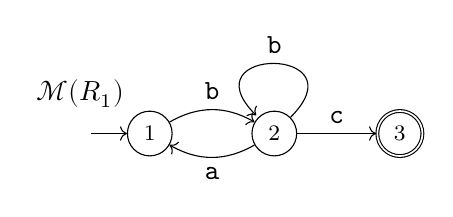
\begin{tikzpicture}
    \tikzset{
      node distance=1cm,
      every state/.append style={minimum size=0.5cm},
      initial text=$ $
    }

    \node[state, initial, label=above left:$\Automaton{\RE{r}_1}$] (s0) {1};
    \node[state, right=of s0] (s1) {2};
    \node[state, accepting, right=of s1] (s2) {3};

    \draw (s0) edge[->, bend left] node[auto]{$\Char{b}$} (s1);
    \draw (s1) edge[->, bend left] node[auto]{$\Char{a}$} (s0);
    \draw (s1) edge[->, loop] node[above]{$\Char{b}$} (s1);
    \draw (s1) edge[->] node[auto]{$\Char{c}$} (s2);
  \end{tikzpicture}
\end{center}

\begin{align*}
  \Automaton{r_1} &= (\Set{Q}_1, \Alphabet, \delta_1, q_{0, 1}, \Set{F}_1)\\[1em]
  \Set{Q}_1 &= \{1, 2, 3\} \\[1em]
  \Alphabet &= \{\Char{a}, \Char{b}, \Char{c}\} \\[1em]
  \delta_1(1, \Char{b}) & =  2\\
  \delta_1(2, \Char{a}) & =  1\\
  \delta_1(2, \Char{b}) & =  2\\
  \delta_1(2, \Char{b}) & =  3\\[1em]
  q_{0, 1} &= 1 \\[1em]
  \Set{F}_1 &= \{3\}
\end{align*}

\begin{center}
\begin{tabular}{ | c | c | c | c | }
   \hline
   $\delta_1$ & \Char{a} & \Char{b} & \Char{c} \\
   \hline
  1 & $\Err$ & 2 & $\Err$  \\
   \hline
  2 & 1 & 2 & 3  \\
   \hline
  3 & $\Err$ & $\Err$ & $\Err$   \\
   \hline
\end{tabular}
\end{center}
\Ex

Vsak regularni izraz lahko ustreza večim različnim avtomatom.

\begin{gather*}
  \RE{r}_2 = \KleenePlus{(\Char{b} \Seq (\Char{a} \Seq \Char{b})?)} \Seq \Char{c} \\
  \Automaton{\RE{r}_2} = (\Set{Q}_2, \Alphabet, \delta_2, q_{0, 2}, \Set{F}_2)
\end{gather*}

\begin{center}
  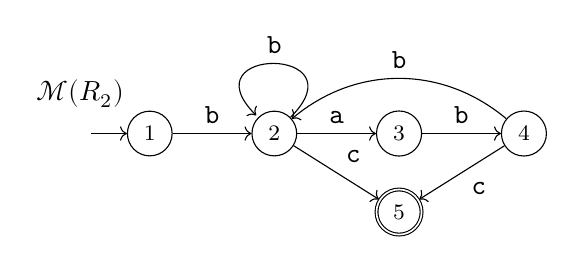
\begin{tikzpicture}
    \tikzset{
      node distance=1cm,
      every state/.append style={minimum size=0.5cm},
      initial text=$ $
    }

    \node[state, initial, label=above left:$\Automaton{\RE{r}_2}$] (s0) {1};
    \node[state, right=of s0] (s1) {2};
    \node[state, right=of s1] (s2) {3};
    \node[state, right=of s2] (s3) {4};
    \node[state, accepting, below=0.4cm of s2] (s4) {5};

    \draw (s0) edge[->] node[auto]{$\Char{b}$} (s1);
    \draw (s1) edge[->, loop] node[above]{$\Char{b}$} (s1);
    \draw (s1) edge[->] node[auto]{$\Char{a}$} (s2);
    \draw (s2) edge[->] node[auto]{$\Char{b}$} (s3);
    \draw (s1) edge[->] node[auto]{$\Char{c}$} (s4);
    \draw (s3) edge[->] node[auto]{$\Char{c}$} (s4);
    \draw (s3) edge[->, bend right=40] node[above]{$\Char{b}$} (s1);
  \end{tikzpicture}
\end{center}

Funkcijo prehodov lahko definiramo tudi za niz:
\begin{align*} % XXX define empty string
  \Kleene{\delta}(q, \varepsilon) &= q\\
  \Kleene{\delta}(q, a \Seq w) &= \Kleene{\delta}(q', w) \text{, kjer } q' = \delta(q, a) \text{ in } q' \neq \Err
\end{align*}

\Ex
\begin{align*}
  \Kleene{\delta_1}(1, \Str{b}) &= 2 \\
  \Kleene{\delta_1}(1, \Str{ba}) &= 1 \\
  \Kleene{\delta_1}(1, \Str{bab}) &= 2 \\
  \Kleene{\delta_1}(1, \Str{bc}) &= 3 \\
  \Kleene{\delta_1}(1, \Str{babbc}) &= 3 \\
  \Kleene{\delta_1}(2, \Str{bbb}) &= 2 \\
  \Kleene{\delta_1}(2, \Str{abbc}) &= 3
\end{align*}

Jezik, ki ga avtomat opisuje:
\begin{equation*}
  \Set{L} = \{w \in \Kleene{\Sigma} \mid \Kleene{\delta}(q_0, w) \in \Set{F}\}
\end{equation*}

\Ex

\begin{align*}
  \Kleene{\delta_1}(1, \Str{bc}) &= 3 \\
  \Kleene{\delta_1}(1, \Str{bbc}) &= 3 \\
  \Kleene{\delta_1}(1, \Str{bbbc}) &= 3 \\
  \cdots \\
  \Kleene{\delta_1}(1, \Str{babc}) &= 3 \\
  \Kleene{\delta_1}(1, \Str{bababc}) &= 3 \\
  \ldots \\
  \Kleene{\delta_1}(1, \Str{babbc}) &= 3 \\
  \Kleene{\delta_1}(1, \Str{babbbc}) &= 3 \\
  \cdots \\
  \Kleene{\delta_1}(1, \Str{bababbc}) &= 3 \\
  \Kleene{\delta_1}(1, \Str{bababbbc}) &= 3 \\
  \cdots \\
\end{align*}

\begin{multline*}
  \Set{L} = \{ \Str{bc}, \Str{bbc}, \Str{bbbc}, \ldots, \Str{babc}, \Str{bababc}, \ldots,\\
  \Str{babbc},  \Str{babbbc}, \ldots, \Str{bababbc}, \Str{bababbbc}, \dots \}
\end{multline*}

%Za implementacijo pregledovalnika je potrebno končnemu avtomatu dodati funkcijo, ki končna stanja preslika v terminale:
%\begin{equation*}
%  \acc: Q \rightarrow T
%\end{equation*}

\section{Konstrukcija}

Za pretvorbo regularnih izrazov v avtomate bomo uporabili konstrukcijo na podlagi deloma razpoznanih regularnih izrazov.
Trenutne pozicije v takšnem regularnem izrazu bodo označene kot $\Pos$.

\Ex Pri $\Char{a} \Seq \Char{b} \Seq \Pos \Char{c} \Seq \Char{d}$ smo že razpoznali $\Str{ab}$ in pričakujemo še $\Str{cd}$.

Za izvedbo konstrukcije potrebujemo naslednje relacije nad deloma razponanimi regularnimi izrazi $(\Move)$, $(\MoveStar)$ in $(\MoveX{\Char{a}})$.
\begin{description}
  \item[$(\Move)$] so pravila za premik trenutnih pozicij v regularnem izrazu skozi operacije.
  \item[$(\MoveStar)$] je zaprtje $(\Move)$. To pomeni, da znova in znova apliciramo pravila $(\Move)$, doker je to mogoče.
  \item[$(\MoveX{\Char{a}})$] so pravila za premik trenutnih pozicij preko znaka $\Char{a}$.
\end{description}

\subsubsection*{Postopek}

Vhod je regularni izraz $\RE{r}$.

Izhod je automat $\Automaton{\RE{r}} = (\Set{Q}, \Set{\Sigma}, \delta, q_{0}, \Set{F})$, ker $\Language{\RE{r}} = \Language{\Automaton{R}}$.

\begin{enumerate}
  \item Začnemo z začetnim stanjem:
    \begin{equation*}
      q_0 = \RE{i}\text{, kjer } \Pos(\RE{r}) \MoveStar \RE{i}
    \end{equation*}
  \item Za vsak znak $\Char{a} \in \Alphabet$, iz trenutnega stanja $q = \RE{i}$ pridobimo stanja:
    \begin{equation*}
      q' = \RE{j}\text{, kjer } \RE{i} \MoveX{\Char{a}} \RE{i}' \MoveStar \RE{j}
    \end{equation*}
    Če že obstaja stanje $q'' = \RE{k}$, kjer $\RE{j} = \RE{k}$, potem $q'$ in $q''$ združimo.
  \item Za vsako stanje dodamo prehod $\delta(q, \Char{a}) = q'$.
  \item Postopek nadaljujemo za vsa tako nastala stanja, ki jih še nismo obravnavali.
  \item Stanje $q = \RE{i}$ je končno, če $\RE{i} = (\RE{r})\Pos$.
\end{enumerate}

\subsection{Prazen jezik}
\begin{tcolorbox}[title={Definicija}]
\begin{equation*}
  \begin{aligned}
    \RE{r} &= \Empty\\
    \Language{\RE{R}} &= \{\}
  \end{aligned}
\end{equation*}
\end{tcolorbox}

\begin{tcolorbox}[title={Konstrukcija}]
\begin{equation*}
  \begin{aligned}
    \Pos\Empty &\Move \Empty
  \end{aligned}
\end{equation*}
\end{tcolorbox}

\begin{center}
  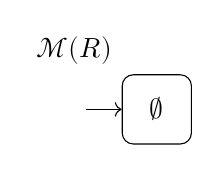
\begin{tikzpicture}
    \tikzset{
      node distance=1cm,
      every state/.style={rectangle, rounded corners, inner sep=0.5em},
      initial text=$ $,
    }
    \node[state, initial, label=above left:$\Automaton{\RE{r}}$] (u0) {$\Empty$};
  \end{tikzpicture}
\end{center}

\subsection{Prazen niz}

\begin{tcolorbox}[title={Definicija}]
\begin{equation*}
  \begin{aligned}
    \RE{r} &= \Null\\
    \Language{\RE{r}} &= \{ \Str{} \}
  \end{aligned}
\end{equation*}
\end{tcolorbox}

\begin{tcolorbox}[title={Konstrukcija}]
\begin{equation*}
  \begin{aligned}
    \Pos\Null &\Move \Null\Pos
  \end{aligned}
\end{equation*}
\end{tcolorbox}

\begin{center}
  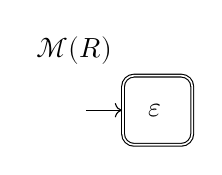
\begin{tikzpicture}
    \tikzset{
      node distance=1cm,
      every state/.style={rectangle, rounded corners, inner sep=0.5em},
      initial text=$ $,
    }
    \node[state, initial, accepting, label=above left:$\Automaton{\RE{r}}$] (u0) {$\Null\Pos$};
  \end{tikzpicture}
\end{center}

Če $\Str{} \in \Language{\RE{r}}$, potem rečemo, da je $\RE{r}$ \emph{nullable}.

\subsection{Znak}

\begin{tcolorbox}[title={Definicija}]
\begin{equation*}
  \begin{aligned}
    \RE{r} &= \Char{a}\text{, kjer } \Char{a} \in \Alphabet\\\
    \Language{\RE{r}} &= \{ \Str{a} \}
  \end{aligned}
\end{equation*}
\end{tcolorbox}

\begin{tcolorbox}[title={Konstrukcija}]
\begin{equation*}
  \begin{aligned}
    \Pos\Char{a} &\MoveX{\Char{a}} \Char{a}\Pos\\
    (\RE{R})\Pos &\MoveX{\Char{a}} \RE{R}\\
    \Pos\Char{a} &\MoveX{\Char{b}} \Char{a}\text{, kjer } \Char{a} \neq \Char{b}
  \end{aligned}
\end{equation*}
\end{tcolorbox}

\begin{center}
  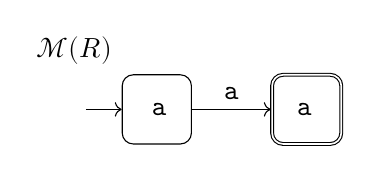
\begin{tikzpicture}
    \tikzset{
      node distance=1cm,
      every state/.style={rectangle, rounded corners, inner sep=0.5em},
      initial text=$ $,
    }
    \node[state, initial, label=above left:$\Automaton{\RE{r}}$] (u0) {$\Pos\Char{a}$};
    \node[state, accepting, right=of u0] (u1) {$\Char{a}\Pos$};
    \draw (u0) edge[->] node[auto]{$\Char{a}$} (u1);
  \end{tikzpicture}
\end{center}

%\begin{equation*}
%  \begin{aligned}
%    \Pos\Set{S} &\MoveX{\Set{S}} \Set{S}\Pos\\
%    %(\RE{R})\Pos &\MoveX{\Char{a}} \RE{R}\\
%    \Pos\Set{S} &\MoveX{\Set{S}} \Set{S}
%  \end{aligned}
%\end{equation*}
%
%\begin{center}
%  \begin{tikzpicture}
%    \tikzset{
%      node distance=1cm,
%      every state/.style={rectangle, rounded corners, inner sep=0.5em},
%      initial text=$ $,
%    }
%    \node[state, initial, label=above left:$\Automaton{R}$] (u0) {$\Pos\Set{S}$};
%    \node[state, right=of u0] (u1) {$\Set{S}\Pos$};
%    \draw (u0) edge[->] node[auto]{$\Set{S}$} (u1);
%  \end{tikzpicture}
%\end{center}

\subsection{Konkatenacija}
\Reset

\begin{tcolorbox}[title={Definicija}]
\begin{equation*}
  \begin{aligned}
    \RE{r} &= \RE{s} \Seq \RE{t} = \RE{s} \Spc \RE{t}\\
    \Language{\RE{r}} &= \{ u \Seq v \mid u \in \Language{\RE{s}} \land v \in \Language{\RE{t}}\}
  \end{aligned}
\end{equation*}
\end{tcolorbox}

\begin{tcolorbox}[title={Pravila}]
\begin{equation*}
  \begin{aligned}
    \RE{s} \Seq \RE{t} &\not= \RE{t} \Seq \RE{s}\\
    \RE{s} \Seq \Null &= \RE{s} \\
    \Null \Seq \RE{s} &= \RE{s} \\
    \RE{s} \Seq \Empty &= \Empty \\
    \Empty \Seq \RE{s} &= \Empty \\
    (\RE{s} \Seq \RE{p}) \Seq \RE{q} &= \RE{s} \Seq (\RE{p} \Seq \RE{q}) = \RE{s} \Seq \RE{p} \Seq \RE{q}
  \end{aligned}
\end{equation*}
\end{tcolorbox}

\vspace{1em}
\Special{Poseben primer:} Če $|\Language{\RE{s}}| = |\Language{\RE{t}}| = 1$, potem $\Language{\RE{s}} = \{u\}$ in $\Language{\RE{t}} = \{v\}$ in $\Language{\RE{r}} = \{u \Seq v\}$.

\Ex
\begin{align*}
  \Language{\RE{s}} &= \{\Str{Hello}\}\\
  \Language{\RE{t}} &= \{\Str{World}\}\\
  \Language{\RE{r}} &= \{\Str{HelloWorld}\}
\end{align*}

Splošno je jezik konkatenacije podoben kartezičnemu produktu.
\begin{align*}
  \Set{S} &= \Set{P} \times \Set{Q} \\
  \Set{S} &= \{ (x, y) \mid x \in \Set{P} \land y \in \Set{Q}\}
\end{align*}

\Ex
\begin{align*}
  \Set{P} &= \{1, 2, 3\}\\
  \Set{Q} &= \{a, b\}\\
  \Set{S} &= \{(1, a), (1, b), (2, a), (2, b), (3, a), (3, b) \}
\end{align*}

Edina razlika je da zamenjamo vsak $(u, v)$, kjer $u \in \Language{\RE{s}}$ in $v\in \Language{\RE{t}}$, z $u \Seq v \in \Language{\RE{r}}$.

\Ex

\begin{align*}
  \RE{P} &= \{\Str{Dober}, \Str{Lep}\}\\
  \RE{Q} &= \{\Str{Dan}, \Str{Večer}, \Str{Tek}\}\\
  \RE{S} &= \{\Str{DoberDan}, \Str{DoberVečer}, \Str{DoberTek}, \Str{LepDan}, \Str{LepVečer}, \Str{LepTek} \}
\end{align*}

\begin{tcolorbox}[title={Konstrukcija}]
  \begin{equation*}
    \begin{aligned}
      \Pos(\RE{R} \Seq \RE{S}) &\Move (\Pos\RE{R}) \Seq \RE{S}\\
      (\RE{R}\Pos) \Seq \RE{S} &\Move \RE{R} \Seq (\Pos \RE{S})\\
      \RE{R} \Seq (\RE{S} \Pos) &\Move (\RE{R} \Seq \RE{S})\Pos
    \end{aligned}
  \end{equation*}
\end{tcolorbox}

\Ex
\begin{align*}
  \N{\RE{r}} &= \Char{a} \Spc \Char{b} \\
\end{align*}
\begin{multline*}
  \Pos(\Char{a} \Seq \Char{b}) \Move (\Pos\Char{a}) \Seq \Char{b} \MoveX{\Char{a}}
  (\Char{a}\Pos) \Seq \Char{b} \Move \Char{a} \Seq (\Pos\Char{b}) \MoveX{\Char{b}}
  \Char{a} \Seq (\Char{b}\Pos) \Move (\Char{a} \Seq \Char{b})\Pos
\end{multline*}
\begin{center}
  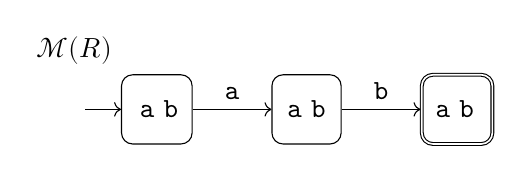
\begin{tikzpicture}
    \tikzset{
      node distance=1cm,
      every state/.style={rectangle, rounded corners, inner sep=0.5em},
      initial text=$ $,
    }

    \node[state, initial, label=above left:$\Automaton{\RE{r}}$] (u0) {$\Pos\Char{a} \Spc \Char{b}$};
    \node[state, right=of u0] (u1) {$\Char{a} \Pos \Char{b}$};
    \node[state, accepting, right=of u1] (u2) {$\Char{a} \Spc \Char{b}\Pos$};
    \draw (u0) edge[->] node[auto]{\Char{a}} (u1);
    \draw (u1) edge[->] node[auto]{\Char{b}} (u2);
  \end{tikzpicture}
\end{center}

\Ex
\begin{align*}
  \N{\RE{r}} &= \Char{a} \Spc \Char{b} \Spc \Char{c} \\
\end{align*}
\begin{multline*}
  \Pos((\Char{a} \Seq \Char{b}) \Seq \Char{c}) \Move
  (\Pos(\Char{a} \Seq \Char{b}) \Seq \Char{c}) \Move
  (((\Pos\Char{a}) \Seq \Char{b}) \Seq \Char{c}) \MoveX{\Char{a}}
  (((\Char{a}\Pos) \Seq \Char{b}) \Seq \Char{c}) \Move
  ((\Char{a} \Seq (\Pos \Char{b})) \Seq \Char{c}) \MoveX{\Char{b}}
  ((\Char{a} \Seq (\Char{b}\Pos)) \Seq \Char{c}) \Move\\
  ((\Char{a} \Seq \Char{b})\Pos \Seq \Char{c}) \Move
  ((\Char{a} \Seq \Char{b}) \Seq (\Pos \Char{c})) \MoveX{\Char{c}}
  ((\Char{a} \Seq \Char{b}) \Seq (\Char{c}\Pos)) \Move
  ((\Char{a} \Seq \Char{b}) \Seq \Char{c})\Pos
\end{multline*}
\begin{center}
  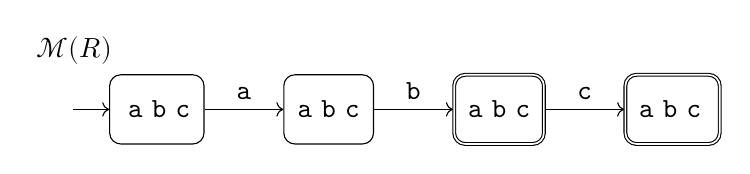
\begin{tikzpicture}
    \tikzset{
      node distance=1cm,
      every state/.style={rectangle, rounded corners, inner sep=0.5em},
      initial text=$ $,
    }

    \node[state, initial, label=above left:$\Automaton{\RE{r}}$] (u0) {$\Pos\Char{a} \Spc \Char{b} \Spc \Char{c}$};
    \node[state, right=of u0] (u1) {$\Char{a} \Pos \Char{b} \Spc \Char{c}$};
    \node[state, accepting, right=of u1] (u2) {$\Char{a} \Spc \Char{b} \Pos \Char{c}$};
    \node[state, accepting, right=of u2] (u3) {$\Char{a} \Spc \Char{b} \Spc \Char{c}\Pos$};
    \draw (u0) edge[->] node[auto]{\Char{a}} (u1);
    \draw (u1) edge[->] node[auto]{\Char{b}} (u2);
    \draw (u2) edge[->] node[auto]{\Char{c}} (u3);
  \end{tikzpicture}
\end{center}

\subsection*{Primeri}

\subsubsection{"then"}
\begin{equation*}
  \Language{\N{\RE{r}}} = \{ \Str{then} \}
\end{equation*}

\subsection{Unija}
\Reset

\begin{tcolorbox}[title={Definicija}]
  \begin{equation*}
    \begin{aligned}
      \RE{r} &= \RE{s} \Union \RE{t} \\
      \Language{\RE{r}} &= \Language{\RE{s}} \cup \Language{\RE{t}}
    \end{aligned}
  \end{equation*}
\end{tcolorbox}

\begin{tcolorbox}[title={Pravila}]
  \begin{equation*}
    \begin{aligned}
      \RE{s} \Union \RE{t} &= \RE{t} \Union \RE{s} \\
      \RE{s} \Union \RE{s} &= \RE{s} \\
      \Empty \Union \RE{s} &= \RE{s} \\
      \RE{s} \Union \Empty &= \RE{s} \\
      (\RE{s} \Union \RE{p}) \Union \RE{q} &= \RE{s} \Union (\RE{p} \Union \RE{q}) = \RE{s} \Union \RE{p} \Union \RE{q} \\
      \RE{s} \Seq (\RE{p} \Union \RE{q}) &= \RE{s} \Seq \RE{p} \Union \RE{s} \Seq \RE{q}\\
      (\RE{p} \Union \RE{q}) \Seq \RE{s} &= \RE{p} \Seq \RE{s} \Union \RE{q} \Seq \RE{s}\\
    \end{aligned}
  \end{equation*}
\end{tcolorbox}

\begin{tcolorbox}[title={Konstrukcija}]
\begin{equation*}
  \begin{aligned}
    \Pos(\RE{R} \Union \RE{S}) &\Move (\Pos\RE{R}) \Union (\Pos\RE{S})\\
    (\RE{R}\Pos) \Union \RE{S} &\Move (\RE{R} \Union \RE{S})\Pos\\
    \RE{R} \Union (\RE{S}\Pos) &\Move (\RE{R} \Union \RE{S})\Pos
  \end{aligned}
\end{equation*}
\end{tcolorbox}

\Ex
\begin{align*}
  \N{\RE{r}} &= \Char{a} \Union \Char{b} \\
\end{align*}
\begin{equation*}
  \Pos(\Char{a} \Union \Char{b}) \Move
  (\Pos\Char{a}) \Union (\Pos\Char{b}) \begin{aligned}[t]
    &\MoveX{\Char{a}} (\Char{a}\Pos) \Union \Char{b} \Move (\Char{a} \Union \Char{b})\Pos \\
    &\MoveX{\Char{b}} \Char{a} \Union (\Char{b}\Pos) \Move (\Char{a} \Union \Char{b})\Pos \\
  \end{aligned}
\end{equation*}
\begin{center}
  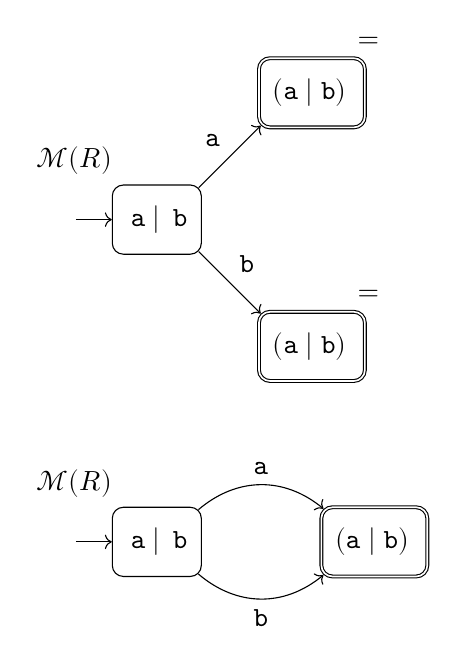
\begin{tikzpicture}
    \tikzset{
      node distance=1cm,
      every state/.style={rectangle, rounded corners, inner sep=0.5em},
      initial text=$ $,
      shorten <>/.style={shorten >=#1, shorten <=#1},
    }

    \node[state, initial, label=above left:$\Automaton{\N{\RE{r}}}$] (u0) {$\Pos\Char{a} \Union \Pos\Char{b}$};
    \node[state, accepting, above right=of u0, label={above right:=}] (u1) {$(\Char{a} \Union \Char{b})\Pos$};

    \draw (u0.north east) edge[->, shorten <>=-2pt+\pgflinewidth] node[auto]{$\Char{a}$} (u1.south west);

    \node[state, accepting, below right=of u0, label={above right:=}] (u4) {$(\Char{a} \Union \Char{b})\Pos$};

    \draw (u0.south east) edge[->, shorten <>=-2pt+\pgflinewidth] node[auto]{$\Char{b}$} (u4.north west);

    \node[state, initial, below=3.2of u0, label=above left:$\Automaton{\N{\RE{r}}}$] (p0) {$\Pos\Char{a} \Union \Pos\Char{b}$};
    \node[state, accepting, right=1.5cm of p0] (p1) {$(\Char{a} \Union \Char{b})\Pos$};

    \draw (p0.north east) edge[->, bend left=40, shorten <>=-2pt+\pgflinewidth] node[auto]{$\Char{a}$} (p1.north west);
    \draw (p0.south east) edge[->, bend right=40, shorten <>=-2pt+\pgflinewidth] node[below]{$\Char{b}$} (p1.south west);

  \end{tikzpicture}
\end{center}

\Ex
\begin{align*}
  \N{\RE{r}} &= \Char{a} \Union \Char{b} \Union \Char{c} \\
\end{align*}
\begin{equation*}
  \Pos((\Char{a} \Union \Char{b}) \Union \Char{c}) \Move
  (\Pos(\Char{a} \Union \Char{b})) \Union (\Pos\Char{c}) \Move
  ((\Pos\Char{a}) \Union (\Pos \Char{b})) \Union (\Pos\Char{c}) \begin{aligned}[t]
    & \MoveX{\Char{a}} ((\Char{a}\Pos) \Union \Char{b}) \Union \Char{c} \Move ((\Char{a} \Union \Char{b}) \Union \Char{c})\Pos \\
    & \MoveX{\Char{b}} (\Char{a} \Union (\Char{b} \Pos)) \Union \Char{c} \Move ((\Char{a} \Union \Char{b}) \Union \Char{c})\Pos \\
    & \MoveX{\Char{c}} (\Char{a} \Union \Char{b}) \Union (\Char{c} \Pos) \Move ((\Char{a} \Union \Char{b}) \Union \Char{c})\Pos 
  \end{aligned}
\end{equation*}

\begin{center}
  \begin{tikzpicture}
    \tikzset{
      node distance=1cm,
      every state/.style={rectangle, rounded corners, inner sep=0.5em},
      initial text=$ $,
      shorten <>/.style={shorten >=#1, shorten <=#1},
    }
    \node[state, initial, below=3.2of u0, label=above left:$\Automaton{\N{R}}$] (p0) {$\Pos\Char{a} \Union \Pos\Char{b} \Union \Pos\Char{c}$};
    \node[state, accepting, right=1.5cm of p0] (p1) {$(\Char{a} \Union \Char{b} \Union \Char{c})\Pos$};

    \draw (p0.north east) edge[->, bend left=40, shorten <>=-2pt+\pgflinewidth] node[auto]{$\Char{a}$} (p1.north west);
    \draw (p0.east) edge[->] node[above]{$\Char{b}$} (p1.west);
    \draw (p0.south east) edge[->, bend right=40, shorten <>=-2pt+\pgflinewidth] node[below]{$\Char{c}$} (p1.south west);
  \end{tikzpicture}
\end{center}

\Ex
\begin{equation*}
  \N{\RE{r}} = \Char{a} \Spc \Char{b} \Union \Char{a} \Spc \Char{b} \Spc \Char{c} \Union \Char{a} \Spc \Char{c} \Spc \Char{d}
\end{equation*}

\begin{center}
  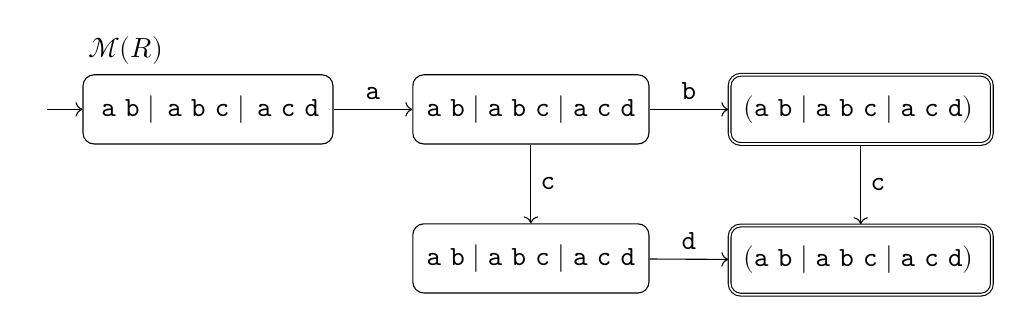
\begin{tikzpicture}
    \tikzset{
      node distance=1cm,
      %every state/.append style={minimum size=0.5cm},
      every state/.style={rectangle, rounded corners, inner sep=0.5em},
      initial text=$ $,
      large/.style={minimum size=1.5cm},
    }

    \node[state, initial, label=above left:$\Automaton{\RE{r}}$] (u0) {$\Pos\Char{a} \Spc \Char{b} \Union \Pos\Char{a}\Spc\Char{b}\Spc\Char{c} \Union \Pos\Char{a}\Spc\Char{c}\Spc\Char{d}$};
    \node[state, right=of u0] (u1) {$\Char{a} \Pos\Char{b} \Union \Char{a}\Pos\Char{b}\Spc\Char{c} \Union \Char{a}\Pos\Char{c}\Spc\Char{d}$};
    \node[state, accepting, right=of u1] (u2) {$(\Char{a} \Spc\Char{b} \Union \Char{a}\Spc\Char{b}\Pos\Char{c} \Union \Char{a}\Spc\Char{c}\Spc\Char{d})\Pos$};
    \draw (u0) edge[->] node[auto]{$\Char{a}$} (u1);
    \draw (u1) edge[->] node[auto]{$\Char{b}$} (u2);

    \node[state, below=of u1] (u4) {$\Char{a} \Spc\Char{b} \Union \Char{a}\Spc\Char{b}\Spc\Char{c} \Union \Char{a}\Spc\Char{c}\Pos\Char{d}$};
    \node[state, accepting, below=of u2] (u3) {$(\Char{a} \Spc\Char{b} \Union \Char{a}\Spc\Char{b}\Spc\Char{c} \Union \Char{a}\Spc\Char{c}\Spc\Char{d})\Pos$};

    \draw (u2) edge[->] node[auto]{$\Char{c}$} (u3);
    \draw (u1) edge[->] node[auto]{$\Char{c}$} (u4);
    \draw (u4) edge[->] node[auto]{$\Char{d}$} (u3);
  \end{tikzpicture}
\end{center}

Avtomat je optimalen.
Ne vemo za katero ključno besedo smo našli ujemanje.

\subsection*{Leva faktorizacija}
Skupno predpono izpostavimo.

\Ex
\begin{align*}
  \N{\RE{r}} &= \Char{a} \Spc \Char{b} \Union \Char{a} \Spc \Char{b} \Spc \Char{c} \Union \Char{a} \Spc \Char{c} \Spc \Char{d}\\
        &= \Char{a} \Seq (\Char{b} \Union \Char{b} \Spc \Char{c} \Union \Char{c} \Spc \Char{d})\\
        &= \Char{a} \Seq (\Char{b} \Seq (\Null \Union \Char{c}) \Union \Char{c} \Spc \Char{d})
\end{align*}

\subsection*{Primeri}
\subsubsection{Ključne besede}

\begin{equation*}
  \N{\RE{r}} = \Char{i} \Spc \Char{f} \Union \Char{f} \Spc \Char{o} \Spc \Char{r} \Union \Char{f} \Spc \Char{o} \Spc \Char{r} \Spc \Char{e} \Spc \Char{a} \Spc \Char{c} \Spc \Char{h}
\end{equation*}

\subsection{Regularne definicije}

\begin{align*}
  \N{\RE{p}} &= \Char{a} \Spc \Char{b}\\
  \N{\RE{q}} &= \Char{a} \Spc \Char{b} \Spc \Char{c}\\
  \N{\RE{t}} &= \Char{a} \Spc \Char{c} \Spc \Char{d}
\end{align*}

\begin{center}
  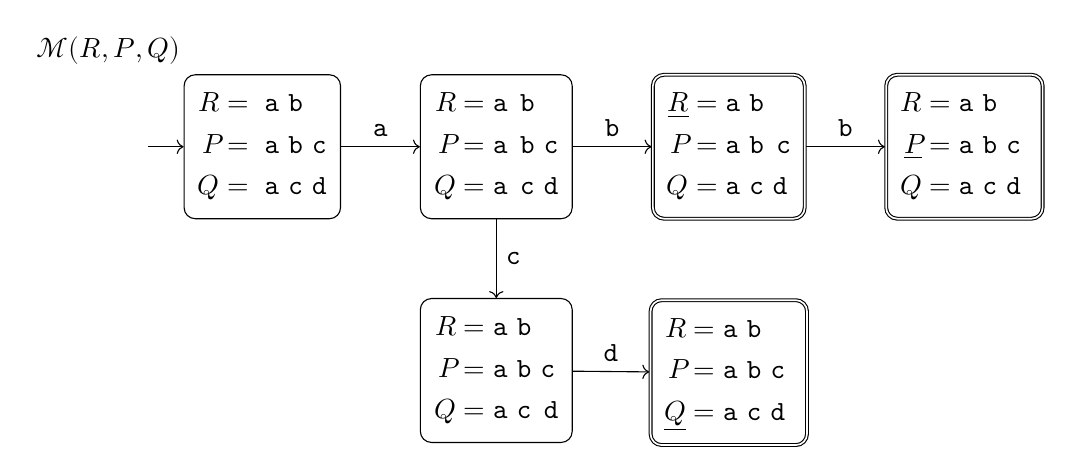
\begin{tikzpicture}
    \tikzset{
      node distance=1cm,
      %every state/.append style={minimum size=0.5cm},
      every state/.style={rectangle, rounded corners, inner sep=0.5em},
      initial text=$ $,
      large/.style={minimum size=1.5cm},
    }

    \node[state, initial, label=above left:$\Automaton{\RE{r}, \RE{p}, \RE{q}}$] (u0) {$\begin{aligned}
      \N{\RE{r}} &= \Pos\Char{a} \Spc \Char{b}\\
      \N{\RE{p}} &= \Pos\Char{a} \Spc \Char{b} \Spc \Char{c}\\
      \N{\RE{q}} &= \Pos\Char{a} \Spc \Char{c} \Spc \Char{d}
    \end{aligned}$};
    \node[state, right=of u0] (u1) {$\begin{aligned}
      \N{\RE{r}} &= \Char{a} \Pos \Char{b}\\
      \N{\RE{p}} &= \Char{a} \Pos \Char{b} \Spc \Char{c}\\
      \N{\RE{q}} &= \Char{a} \Pos \Char{c} \Spc \Char{d}
    \end{aligned}$};
    \node[state, accepting, right=of u1] (u2) {$\begin{aligned}
      \underline{\N{\RE{r}}} &= \Char{a} \Spc \Char{b}\Pos\\
      \N{\RE{p}} &= \Char{a} \Spc \Char{b} \Pos \Char{c}\\
      \N{\RE{q}} &= \Char{a} \Spc \Char{c} \Spc \Char{d}
    \end{aligned}$};
    \node[state, accepting, right=of u2] (u5) {$\begin{aligned}
      \N{\RE{r}} &= \Char{a} \Spc \Char{b}\\
      \underline{\N{\RE{p}}} &= \Char{a} \Spc \Char{b} \Spc \Char{c}\Pos\\
      \N{\RE{q}} &= \Char{a} \Spc \Char{c} \Spc \Char{d}
    \end{aligned}$};

    \draw (u0) edge[->] node[auto]{$\Char{a}$} (u1);
    \draw (u1) edge[->] node[auto]{$\Char{b}$} (u2);
    \draw (u2) edge[->] node[auto]{$\Char{b}$} (u5);

    \node[state, below=of u1] (u4) {$\begin{aligned}
      \N{\RE{r}} &= \Char{a} \Spc \Char{b}\\
      \N{\RE{p}} &= \Char{a} \Spc \Char{b} \Spc \Char{c}\\
      \N{\RE{q}} &= \Char{a} \Spc \Char{c} \Pos \Char{d}
    \end{aligned}$};

    \node[state, accepting, below=of u2] (u3) {$\begin{aligned}
      \N{\RE{r}} &= \Char{a} \Spc \Char{b}\\
      \N{\RE{p}} &= \Char{a} \Spc \Char{b} \Spc \Char{c}\\
      \underline{\N{\RE{q}}} &= \Char{a} \Spc \Char{c} \Spc \Char{d} \Pos
    \end{aligned}$};

    \draw (u1) edge[->] node[auto]{$\Char{c}$} (u4);
    \draw (u4) edge[->] node[auto]{$\Char{d}$} (u3);
  \end{tikzpicture}
\end{center}

Nastali avtomat je drevo predpon.

\subsection*{Primeri}
\subsubsection{Ključne besede}

\begin{align*}
  \N{\RE{p}} &= \Char{i} \Spc \Char{f} \\
  \N{\RE{q}} &= \Char{f} \Spc \Char{o} \Spc \Char{r} \\
  \N{\RE{t}} &= \Char{f} \Spc \Char{o} \Spc \Char{r} \Spc \Char{e} \Spc \Char{a} \Spc \Char{c} \Spc \Char{h} \\
\end{align*}

\subsection{Množica znakov}
\Reset

\begin{tcolorbox}[title={Definicija}]
\begin{equation*}
  \begin{aligned}
    R &= \Set{S}\text{, kjer } \Set{S} \subseteq \Alphabet \\
    &= \Char{a} \Union \dots \Union \Char{b}\text{, kjer } \Char{a}, \dots, \Char{b} \in \Set{S}\\
    \Language{\RE{r}} &= \Set{S}
  \end{aligned}
\end{equation*}
\end{tcolorbox}

Množica znakov se lahko predstavi kot šop prehodov (eden za vsak znak) ali pa en sam prehod označen z množico.

\Ex
\begin{align*}
  \N{\RE{r}} &= \Char{a} \Union \Char{b} = \{\Char{a}, \Char{b}\} \\
\end{align*}
\begin{center}
  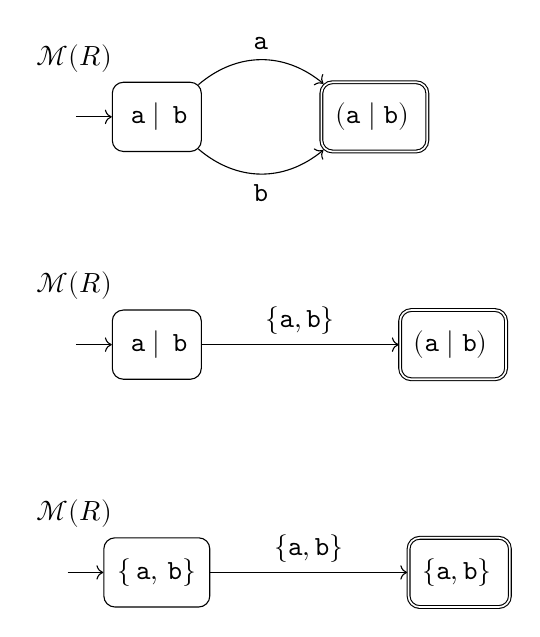
\begin{tikzpicture}
    \tikzset{
      node distance=1cm,
      every state/.style={rectangle, rounded corners, inner sep=0.5em},
      initial text=$ $,
      shorten <>/.style={shorten >=#1, shorten <=#1},
    }

    \node[state, initial, label=above left:$\Automaton{\N{\RE{r}}}$] (p0) {$\Pos\Char{a} \Union \Pos\Char{b}$};
    \node[state, accepting, right=1.5cm of p0] (p1) {$(\Char{a} \Union \Char{b})\Pos$};

    \draw (p0.north east) edge[->, bend left=40, shorten <>=-2pt+\pgflinewidth] node[auto]{$\Char{a}$} (p1.north west);
    \draw (p0.south east) edge[->, bend right=40, shorten <>=-2pt+\pgflinewidth] node[below]{$\Char{b}$} (p1.south west);

    \node[state, initial, below=2of p0, label=above left:$\Automaton{\N{\RE{r}}}$] (q0) {$\Pos\Char{a} \Union \Pos\Char{b}$};
    \node[state, accepting, right=2.5cm of q0] (q1) {$(\Char{a} \Union \Char{b})\Pos$};

    \draw (q0) edge[->] node[auto]{$\{\Char{a}, \Char{b}\}$} (q1);

    \node[state, initial, below=2of q0, label=above left:$\Automaton{\N{\RE{r}}}$] (t0) {$\{\Pos\Char{a}, \Pos\Char{b}\}$};
    \node[state, accepting, right=2.5cm of t0] (t1) {$\{\Char{a}, \Char{b}\}\Pos$};

    \draw (t0) edge[->] node[auto]{$\{\Char{a}, \Char{b}\}$} (t1);
  \end{tikzpicture}
\end{center}

\Ex
\begin{align*}
  \N{\RE{r}} &= \{\Char{a}, \Char{b}\}\\
  \N{\RE{s}} &= \{\Char{b}, \Char{c}, \Char{d}\}
\end{align*}

\begin{center}
  \begin{tikzpicture}
    \tikzset{
      node distance=1cm,
      every state/.style={rectangle, rounded corners, inner sep=0.5em},
      initial text=$ $,
      shorten <>/.style={shorten >=#1, shorten <=#1},
    }

    \node[state, initial, below=2of q0, label=above left:$\Automaton{\N{\RE{r}}, \N{\RE{s}}}$] (t0) {$\begin{aligned}\RE{r} &= \{\Pos\Char{a}, \Pos\Char{b}\}\\ \RE{s} &= \{\Pos\Char{b}, \Pos\Char{c}, \Pos\Char{d}\}\end{aligned}$};
    \node[state, accepting, above right=2.5cm of t0] (t1) {$\begin{aligned}\RE{r} &= \{\Char{a}, \Char{b}\}\Pos\\ \RE{s} &= \{\Char{b}, \Char{c}, \Char{d}\}\end{aligned}$};
    \node[state, accepting, right=2.5cm of t0] (t2) {$\begin{aligned}\RE{r} &= \{\Char{a}, \Char{b}\}\Pos\\ \RE{s} &= \{\Char{b}, \Char{c}, \Char{d}\}\Pos\end{aligned}$};
    \node[state, accepting, below right=2.5cm of t0] (t3) {$\begin{aligned}\RE{r} &= \{\Char{a}, \Char{b}\}\\ \RE{s} &= \{\Char{b}, \Char{c}, \Char{d}\}\Pos\end{aligned}$};

    \draw (t0.north east) edge[->, shorten <>=-2pt+\pgflinewidth] node[auto]{$\{\Char{a}\}$} (t1.south west);
    \draw (t0) edge[->] node[auto]{$\{\Char{b}\}$} (t2);
    \draw (t0.south east) edge[->, shorten <>=-2pt+\pgflinewidth] node[auto]{$\{\Char{c}, \Char{d}\}$} (t3.north west);
  \end{tikzpicture}
\end{center}
Paziti moramo, da avtomat ne postane nedeterminističen.

\subsection*{Primeri}

\subsubsection{Y/N}

\begin{equation*}
  \Language{\N{\RE{r}}} = \{ \Str{Y}, \Str{N} \}
\end{equation*}

\begin{equation*}
  \N{\RE{r}} = \{ \Char{Y}, \Char{N} \}
\end{equation*}

\begin{center}
  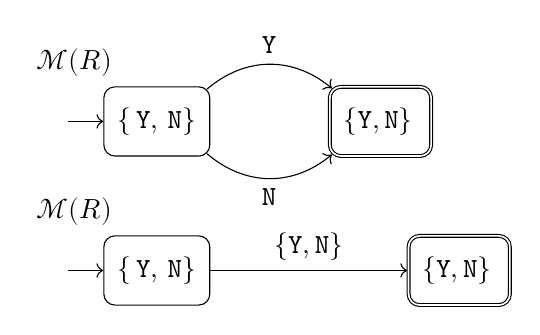
\begin{tikzpicture}
    \tikzset{
      node distance=1cm,
      every state/.style={rectangle, rounded corners, inner sep=0.5em},
      initial text=$ $,
      shorten <>/.style={shorten >=#1, shorten <=#1},
    }

    \node[state, initial, label=above left:$\Automaton{\N{\RE{r}}}$] (p0) {$\{ \Pos\Char{Y}, \Pos\Char{N} \}$};
    \node[state, accepting, right=1.5cm of p0] (p1) {$\{ \Char{Y}, \Char{N} \}\Pos$};

    \node[state, initial, below=of p0, label=above left:$\Automaton{\N{\RE{r}}}$] (q0) {$\{ \Pos\Char{Y}, \Pos\Char{N} \}$};
    \node[state, accepting, right=2.5cm of q0] (q1) {$\{ \Char{Y}, \Char{N} \}\Pos$};


    \draw (q0) edge[->] node[auto]{$\{\Char{Y}, \Char{N} \} $} (q1);

    \draw (p0.north east) edge[->, bend left=40, shorten <>=-2pt+\pgflinewidth] node[auto]{$\Char{Y}$} (p1.north west);
    \draw (p0.south east) edge[->, bend right=40, shorten <>=-2pt+\pgflinewidth] node[below]{$\Char{N}$} (p1.south west);
  \end{tikzpicture}
\end{center}
\Next

\subsubsection{Števke}

\begin{equation*}
  \Language{\N{\RE{r}}} = \{ \Str{0}, \Str{1}, \Str{2}, \dots, \Str{9} \}
\end{equation*}

\begin{equation*}
  \N{\RE{r}} = \{ \Char{0}, \Char{1}, \Char{2}, \dots, \Char{9} \}
\end{equation*}

\begin{center}
  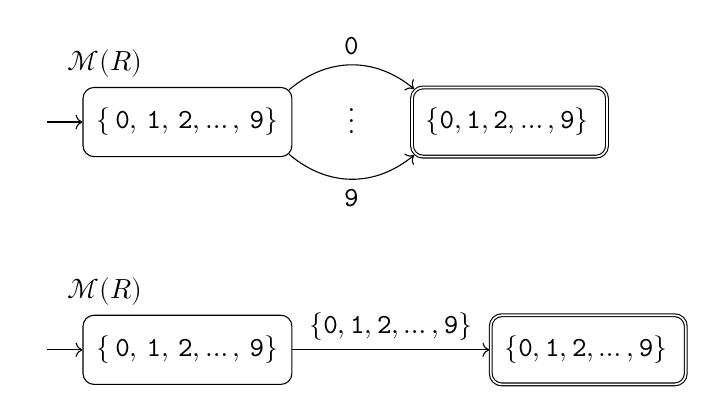
\begin{tikzpicture}
    \tikzset{
      node distance=1cm,
      every state/.style={rectangle, rounded corners, inner sep=0.5em},
      initial text=$ $,
      shorten <>/.style={shorten >=#1, shorten <=#1},
    }

    \node[state, initial, label=above left:$\Automaton{\N{\RE{r}}}$] (p0) {$\{ \Pos\Char{0}, \Pos\Char{1}, \Pos\Char{2}, \dots, \Pos\Char{9} \}$};
    \node[state, accepting, right=1.5cm of p0] (p1) {$\{ \Char{0}, \Char{1}, \Char{2}, \dots, \Char{9} \}\Pos$};
    \node at ($(p0.east)!0.5!(p1.west)$) {\Dots{}};

    \node[state, initial, below=2of p0, label=above left:$\Automaton{\N{\RE{r}}}$] (q0) {$\{ \Pos\Char{0}, \Pos\Char{1}, \Pos\Char{2}, \dots, \Pos\Char{9} \}$};
    \node[state, accepting, right=2.5cm of q0] (q1) {$\{ \Char{0}, \Char{1}, \Char{2}, \dots, \Char{9} \} \Pos$};


    \draw (q0) edge[->] node[auto]{$\{\Char{0}, \Char{1}, \Char{2}, \ldots, \Char{9} \} $} (q1);

    \draw (p0.north east) edge[->, bend left=40, shorten <>=-2pt+\pgflinewidth] node[auto]{$\Char{0}$} (p1.north west);
    \draw (p0.south east) edge[->, bend right=40, shorten <>=-2pt+\pgflinewidth] node[below]{$\Char{9}$} (p1.south west);
  \end{tikzpicture}
\end{center}
\Next

\subsubsection{Male črke}

\begin{equation*}
  \Language{\N{\RE{r}}} = \{ \Str{a}, \Str{b}, \Str{c}, \dots, \Str{z} \}
\end{equation*}
\Next

\subsubsection{Velike in male črke}

\begin{equation*}
  \Language{\N{\RE{r}}} = \{ \Str{A}, \Str{B}, \Str{C}, \dots, \Str{Z}, \Str{a}, \Str{b}, \Str{c}, \dots, \Str{z} \}
\end{equation*}
\Next

\subsubsection{Heksadecimalne števke}


\begin{equation*}
  \Language{\N{\RE{r}}} = \{ \Str{0}, \Str{1}, \Str{2}, \dots, \Str{9}, \Str{A}, \dots, \Str{F} \}
\end{equation*}

\subsubsection{"then", "Then", "THEN", "theN", ...}
\begin{equation*}
  \N{\RE{r}} = \{\Char{T}, \Char{t}\} \Seq \{\Char{H}, \Char{h}\} \Seq \{\Char{E}, \Char{e}\} \Seq \{\Char{N}, \Char{n}\}
\end{equation*}

\Next
\subsubsection{Bajt po osmiško}

\begin{equation*}
  \N{\RE{r}} = \{\Char{0}, \dots, \Char{3}\} \Seq \{\Char{0}, \dots, \Char{7}\} \Seq \{\Char{0}, \dots, \Char{7}\}
\end{equation*}

\begin{equation*}
  \Language{\N{\RE{r}}} = \{ \Str{000}, \Str{001}, \Str{002}, \dots, \Str{377} \}
\end{equation*}
\Next

\subsection{Opcija}
\Reset

\begin{tcolorbox}[title={Definicija}]
  \begin{equation*}
    \begin{aligned}
      \Opt{\RE{s}} &= \Null \Union \RE{s}\\
      \Language{\Opt{\RE{s}}} &= \{\Str{}\} \cup \Language{\RE{s}}
    \end{aligned}
  \end{equation*}
\end{tcolorbox}

Ujemanje $S$ 0 ali 1 krat.

\begin{tcolorbox}[title={Konstrukcija}]
\begin{equation*}
  \begin{aligned}
    \Pos(\Opt{\RE{R}}) &\Move (\Opt{(\Pos\RE{R})})\Pos\\
    \Opt{(\RE{R}\Pos)} &\Move (\Opt{\RE{R}})\Pos
  \end{aligned}
\end{equation*}
\end{tcolorbox}

\Ex
\begin{align*}
  \N{\RE{s}} &= \Char{a}\\
  \N{\RE{r}} &= \Opt{\Char{a}}
\end{align*}
\begin{align*}
  \Language{\N{\RE{s}}} &= \{ \Str{a} \}\\
  \Language{\N{\RE{r}}} &= \{ \Str{}, \Str{a} \}
\end{align*}

\begin{equation*}
  \Pos(\Opt{\Char{a}}) \Move
  (\Opt{(\Pos\Char{a})})\Pos \MoveX{\Char{a}}
  \Opt{(\Char{a}\Pos)} \Move
  (\Opt{\Char{a}})\Pos
\end{equation*}
\begin{center}
  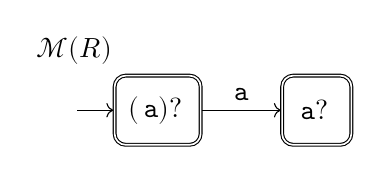
\begin{tikzpicture}
    \tikzset{
      node distance=1cm,
      every state/.style={rectangle, rounded corners, inner sep=0.5em},
      initial text=$ $,
    }
    \node[state, initial, accepting, label=above left:$\Automaton{R}$] (u0) {$\Opt{(\Pos\Char{a})}\Pos$};
    \node[state, accepting, right=of u0] (u1) {$\Opt{\Char{a}}\Pos$};
    \draw (u0) edge[->] node[auto]{$\Char{a}$} (u1);
  \end{tikzpicture}
\end{center}

\Ex
\begin{align*}
  \N{\RE{s}} &= \Char{a} \Seq \Char{b}\\
  \N{\RE{r}} &= \Opt{(\Char{a} \Seq \Char{b})}
\end{align*}
\begin{align*}
  \Language{\N{\RE{s}}} &= \{\Str{ab}\} \\
  \Language{\N{\RE{r}}} &= \{\Str{}, \Str{ab}\}
\end{align*}
\begin{multline*}
  \Pos(\Opt{(\Char{a} \Seq \Char{b})}) \Move
  (\Opt{\Pos(\Char{a} \Seq \Char{b})})\Pos \Move
  (\Opt{((\Pos\Char{a}) \Seq \Char{b})})\Pos \MoveX{\Char{a}}
  \Opt{((\Char{a}\Pos) \Seq \Char{b})} \Move\\
  \Opt{(\Char{a} \Seq (\Pos\Char{b}))} \MoveX{\Char{b}}
  \Opt{(\Char{a} \Seq (\Char{b}\Pos))} \Move
  \Opt{((\Char{a} \Seq \Char{b})\Pos)} \Move
  (\Opt{(\Char{a} \Seq \Char{b})})\Pos
\end{multline*}
\begin{center}
  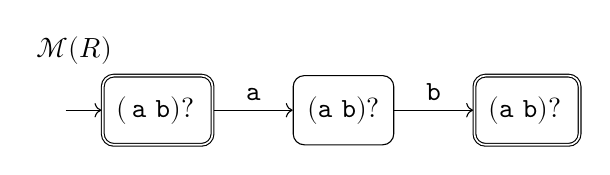
\begin{tikzpicture}
    \tikzset{
      node distance=1cm,
      every state/.style={rectangle, rounded corners, inner sep=0.5em},
      initial text=$ $,
    }
    \node[state, initial, accepting, label=above left:$\Automaton{R}$] (u0) {$\Opt{(\Pos\Char{a} \Spc \Char{b})}\Pos$};
    \node[state, right=of u0] (u1) {$\Opt{(\Char{a} \Pos \Char{b})}$};
    \node[state, accepting, right=of u1] (u2) {$\Opt{(\Char{a} \Spc \Char{b})}\Pos$};
    \draw (u0) edge[->] node[auto]{$\Char{a}$} (u1);
    \draw (u1) edge[->] node[auto]{$\Char{b}$} (u2);
  \end{tikzpicture}
\end{center}

\subsection{Potence}
\Reset

\begin{tcolorbox}[title={Definicija}]
\begin{equation*}
  \begin{aligned}
    \Rep{\RE{s}}{0} &= \Null\\
    \Rep{\RE{s}}{i+1} &= \Rep{\RE{s}}{i} \Seq \RE{s}\\[1em]
    \Rep{\RE{s}}{i} &= \underbrace{\RE{s} \Seq \ldots \Seq \RE{s}}_{i}\\[1em]
    \Language{\Rep{\RE{s}}{0}} &= \Null\\
    \Language{\Rep{\RE{s}}{i+1}} &= \{u \Seq v \mid u \in \Language{\Rep{\RE{s}}{i}} \land v \in \Language{\RE{s}}\}
  \end{aligned}
\end{equation*}
\end{tcolorbox}
\begin{align*}
\end{align*}

%\begin{tcolorbox}[title={Konstrukcija}]
%\begin{equation*}
%  \begin{aligned}
%    \Pos(\Rep{\RE{R}}{n}) &\Move \Rep{(\Pos\RE{R})}{n}\\
%    \Rep{(\RE{R}\Pos)}{n} &\Move \Rep{(\Pos\RE{R})}{n-1}\\
%    \Rep{(\Pos\RE{R})}{0} &\Move (\Rep{\RE{R}}{0})\Pos
%  \end{aligned}
%\end{equation*}
%\end{tcolorbox}

\Ex
\begin{align*}
  \N{\RE{s}} &= \Char{a}\\
  \N{\RE{r}} &= \Rep{\Char{a}}{2} = \Char{a} \Seq \Char{a}
\end{align*}

\begin{align*}
  \Language{\N{\RE{s}}} &= \{ \Str{a} \}\\
  \Language{\N{\RE{r}}} &= \{ \Str{aa} \}
\end{align*}

\begin{center}
  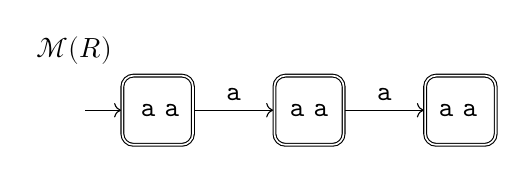
\begin{tikzpicture}
    \tikzset{
      node distance=1cm,
      every state/.style={rectangle, rounded corners, inner sep=0.5em},
      initial text=$ $,
    }
    \node[state, initial, accepting, label=above left:$\Automaton{R}$] (u0) {$\Pos\Char{a} \Spc \Char{a}$};
    \node[state, accepting, right=of u0] (u1) {$\Char{a} \Pos \Char{a}$};
    \node[state, accepting, right=of u1] (u2) {$\Char{a} \Spc \Char{a}\Pos$};
    \draw (u0) edge[->] node[auto]{$\Char{a}$} (u1);
    \draw (u1) edge[->] node[auto]{$\Char{a}$} (u2);
  \end{tikzpicture}
\end{center}

\subsection*{Primeri}

\subsubsection{"aaaa"}

\begin{align*}
  \N{\RE{s}} &= \Char{a} \\
  \N{\RE{r}} &= \Char{a}^4
\end{align*}
\begin{align*}
  \Language{\N{\RE{s}}} &= \{\Str{a}\} \\
  \Language{\N{\RE{r}}} &= \{\Str{aaaa}\}
\end{align*}
\Next

\subsubsection{"abab"}

\begin{align*}
  \N{\RE{s}} &= \Char{a} \Spc \Char{b} \\
  \N{\RE{r}} &= (\Char{a} \Spc \Char{b})^2
\end{align*}
\begin{align*}
  \Language{\N{\RE{s}}} &= \{\Str{ab}\} \\
  \Language{\N{\RE{r}}} &= \{\Str{abab}\}
\end{align*}
\Next

\subsubsection{Bajt po osmiško}
\begin{equation*}
  \N{\RE{r}} = \{\Char{0}, \dots, \Char{3}\} \Seq (\{\Char{0}, \dots, \Char{7}\})^2
\end{equation*}
\Next

\subsection{Kleene-ovo zaprtje}
\Reset

\begin{tcolorbox}[title={Definicija}]
  \begin{equation*}
    \begin{aligned}
      \Kleene{\RE{s}} &= \Null \Union \RE{s} \Union \RE{s} \Seq \RE{s} \Union \RE{s} \Seq \RE{s} \Seq \RE{s} \Union \ldots \\
      &= \Rep{\RE{s}}{0} \Union \Rep{\RE{s}}{1} \Union \Rep{\RE{s}}{2} \Union \ldots \\
      &= \Big\vert_{i = 0}^\infty \Rep{\RE{s}}{i}\\
      \Language{\Kleene{\RE{s}}} &= \bigcup_{i = 0}^\infty \Language{\RE{s}^i}
    \end{aligned}
  \end{equation*}
\end{tcolorbox}

Ujemanje $s$ 0 ali več krat.
Z drugimi besedami, $s$ je lahko ponovljen $0, 1, 2, \dots, \infty$ krat.

\begin{tcolorbox}[title={Pravila}]
  \begin{equation*}
    \begin{aligned}
      \Kleene{\Empty} &= \Null\\
      \Kleene{\Null} &= \Null\\
      \Null \Union \Kleene{\RE{s}} &= \Kleene{\RE{s}}\\
      \Kleene{\RE{s}} \Union \Null &= \Kleene{\RE{s}}\\
      \Kleene{(\Kleene{\RE{s}})} &= \Kleene{\RE{s}}\\
      \Kleene{(\RE{s} \Union \RE{t})} &= \Kleene{(\Kleene{\RE{s}} \Seq \RE{t})} \Seq \Kleene{\RE{s}}\\
      \Kleene{(\RE{s} \Seq \RE{t})} &= \Null \Union \RE{s} \Seq \Kleene{(\RE{t} \Seq \RE{s})} \Seq \RE{t}\\
      \Kleene{\RE{s}} &= (\Null \Union \RE{s} \Union ... \Union \Rep{\RE{s}}{i - 1}) \Seq \Kleene{(\Rep{\RE{s}}{i})}
    \end{aligned}
  \end{equation*}
\end{tcolorbox}

\begin{tcolorbox}[title={Konstrukcija}]
\begin{equation*}
  \begin{aligned}
    \Pos(\Kleene{\RE{R}}) &\Move (\Kleene{(\Pos\RE{R})})\Pos\\
    \Kleene{(\RE{R}\Pos)} &\Move (\Kleene{(\Pos\RE{R})})\Pos
  \end{aligned}
\end{equation*}
\end{tcolorbox}

\Ex
\begin{align*}
  \N{\RE{s}} &= \Char{a}\\
  \N{\RE{r}} &= \Kleene{\Char{a}}
\end{align*}

\begin{align*}
  \Language{\N{\RE{s}}} &= \{\Str{a}\}\\
  \Language{\N{\RE{r}}} &= \{\Str{}, \Str{a}, \Str{aa}, \Str{aaa}, \dots\}
\end{align*}

\begin{equation*}
  \Pos(\Kleene{\Char{a}}) \Move
  (\Kleene{(\Pos\Char{a})})\Pos \MoveX{\Char{a}}
  \Kleene{(\Char{a}\Pos)} \Move
  (\Kleene{(\Pos\Char{a})})\Pos \MoveX{\Char{a}} \cdots
\end{equation*}
\begin{center}
  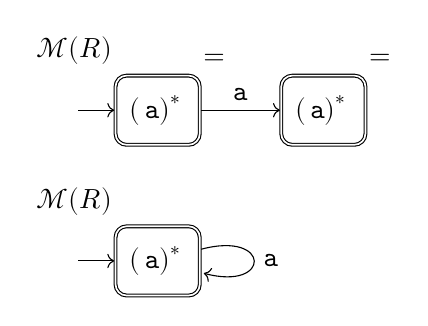
\begin{tikzpicture}
    \tikzset{
      node distance=1cm,
      every state/.style={rectangle, rounded corners, inner sep=0.5em},
      initial text=$ $,
    }
    \node[state, initial, accepting, label=above left:$\Automaton{\RE{r}}$, label={above right:=}] (u0) {$\Kleene{(\Pos\Char{a})}\Pos$};
    \node[state, accepting, right=of u0, label={above right:=}] (u1) {$\Kleene{(\Pos\Char{a})}\Pos$};
    \draw (u0) edge[->] node[auto]{$\Char{a}$} (u1);

    \node[state, initial, below=of u0, accepting, label=above left:$\Automaton{\RE{r}}$] (p0) {$\Kleene{(\Pos\Char{a})}\Pos$};
    \draw (p0) edge[->, loop right] node[auto]{$\Char{a}$} (p0);
  \end{tikzpicture}
\end{center}

\Ex
\begin{align*}
  \N{\RE{s}} &= \Char{a} \Spc \Char{b} \\
  \N{\RE{r}} &= \Kleene{(\Char{a} \Spc \Char{b})}
\end{align*}

\begin{align*}
  \Language{\N{\RE{s}}} &= \{\Str{ab}\} \\
  \Language{\N{\RE{r}}} &= \{\Str{}, \Str{ab}, \Str{abab}, \Str{ababab}, \dots\}
\end{align*}

\begin{center}
  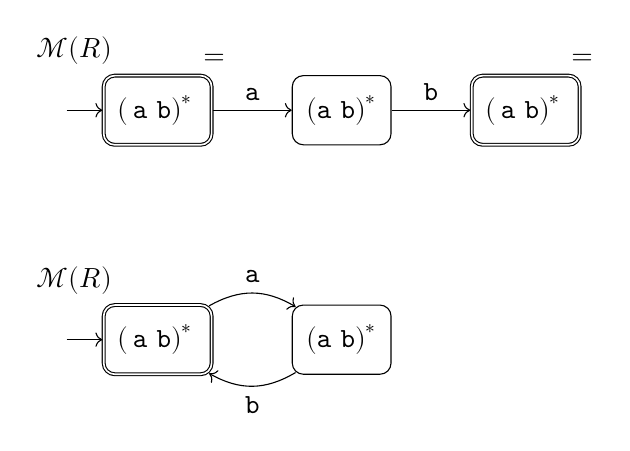
\begin{tikzpicture}
    \tikzset{
      node distance=1cm,
      every state/.style={rectangle, rounded corners, inner sep=0.5em},
      initial text=$ $,
      shorten <>/.style={shorten >=#1, shorten <=#1},
    }
    \node[state, initial, accepting, label=above left:$\Automaton{\RE{r}}$, label={above right:=}] (u0) {$\Kleene{(\Pos\Char{a}\Spc\Char{b})}\Pos$};
    \node[state, right=of u0] (u1) {$\Kleene{(\Char{a}\Pos\Char{b})}$};
    \node[state, accepting, right=of u1, label={above right:=}] (u2) {$\Kleene{(\Pos\Char{a}\Spc\Char{b})}\Pos$};
    \draw (u0) edge[->] node[auto]{$\Char{a}$} (u1);
    \draw (u1) edge[->] node[auto]{$\Char{b}$} (u2);

    \node[state, initial, accepting, below=2 of u0, label=above left:$\Automaton{\RE{r}}$] (p0) {$\Kleene{(\Pos\Char{a}\Spc\Char{b})}\Pos$};
    \node[state, right=of p0] (p1) {$\Kleene{(\Char{a}\Pos\Char{b})}$};
    \draw (p0.north east) edge[->, bend left, shorten <>=-2pt+\pgflinewidth] node[auto]{$\Char{a}$} (p1.north west);
    \draw (p1.south west) edge[->, bend left, shorten <>=-2pt+\pgflinewidth] node[auto]{$\Char{b}$} (p0.south east);
  \end{tikzpicture}
\end{center}

\Ex

\begin{equation*}
  \N{\RE{r}} = \Char{c} \Spc \Kleene{(\Char{a} \Spc \Char{b})}
\end{equation*}

\begin{equation*}
  \Language{\N{\RE{r}}} = \{\Str{c}, \Str{cab}, \Str{cabab}, \Str{cababab}, \dots\}
\end{equation*}

\begin{center}
  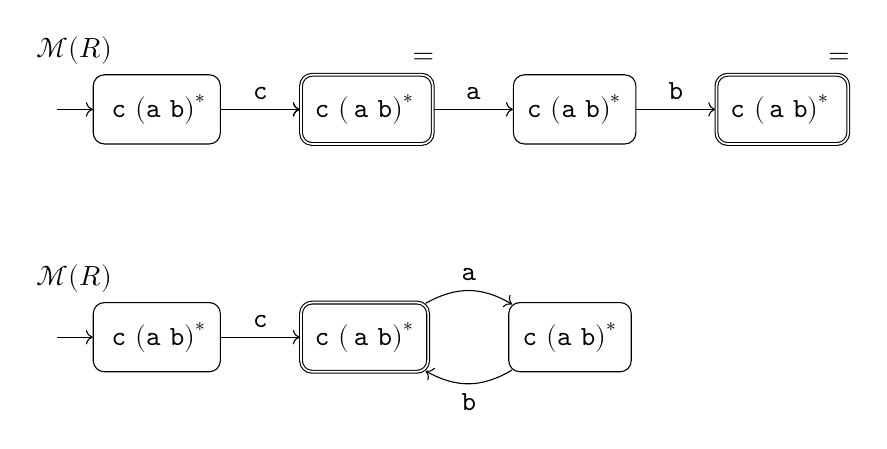
\begin{tikzpicture}
    \tikzset{
      node distance=1cm,
      every state/.style={rectangle, rounded corners, inner sep=0.5em},
      initial text=$ $,
      shorten <>/.style={shorten >=#1, shorten <=#1},
    }
    \node[state, initial, label=above left:$\Automaton{\RE{r}}$] (u0) {$\Pos\Char{c} \Spc \Kleene{(\Char{a} \Spc \Char{b})}$};
    \node[state, initial, accepting, right=of u0, label={above right:=}] (u1) {$\Char{c} \Spc \Kleene{(\Pos\Char{a} \Spc \Char{b})}\Pos$};
    \node[state, right=of u1] (u2) {$\Char{c} \Spc \Kleene{(\Char{a} \Pos \Char{b})}$};
    \node[state, accepting, right=of u2, label={above right:=}] (u3) {$\Char{c} \Spc \Kleene{(\Pos\Char{a} \Spc \Char{b})}\Pos$};
    \draw (u0) edge[->] node[auto]{$\Char{c}$} (u1);
    \draw (u1) edge[->] node[auto]{$\Char{a}$} (u2);
    \draw (u2) edge[->] node[auto]{$\Char{b}$} (u3);

    \node[state, initial, below=2 of u0, label=above left:$\Automaton{\RE{r}}$] (p0) {$\Pos\Char{c} \Spc \Kleene{(\Char{a}\Spc\Char{b})}$};
    \node[state, accepting, right=of p0] (p1) {$\Char{c} \Spc \Kleene{(\Pos\Char{a}\Spc\Char{b})}$};
    \node[state, right=of p1] (p2) {$\Char{c} \Spc \Kleene{(\Char{a}\Pos\Char{b})}$};
    \draw (p0) edge[->] node[auto]{$\Char{c}$} (p1);
    \draw (p1.north east) edge[->, bend left, shorten <>=-2pt+\pgflinewidth] node[auto]{$\Char{a}$} (p2.north west);
    \draw (p2.south west) edge[->, bend left, shorten <>=-2pt+\pgflinewidth] node[auto]{$\Char{b}$} (p1.south east);
  \end{tikzpicture}
\end{center}
\Next

\Ex
\begin{equation*}
  \N{\RE{r}} = \Kleene{(\Char{a} \Spc \Char{a} \Union \Char{b})}
\end{equation*}

\begin{equation*}
  \Language{\N{\RE{r}}} = \{\Null, \Str{b}, \Str{aa}, \Str{bb}, \Str{aab}, \Str{baa}, \Str{aaaa}, \dots\}
\end{equation*}

\begin{center}
  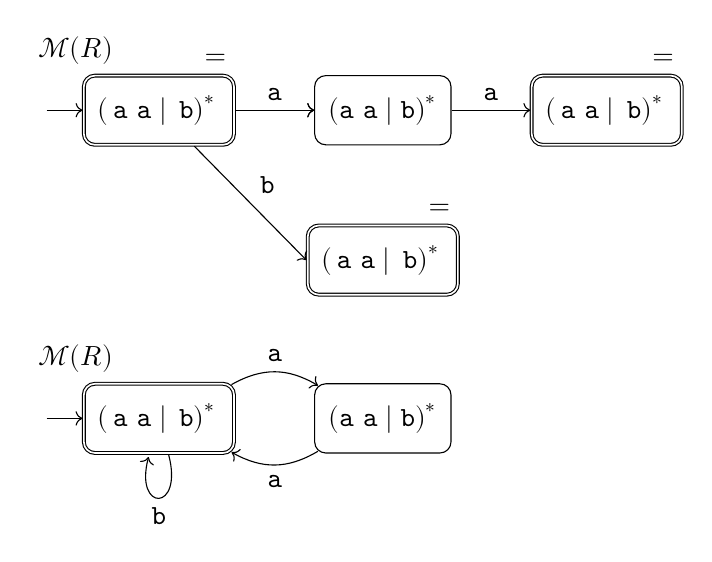
\begin{tikzpicture}
    \tikzset{
      node distance=1cm,
      every state/.style={rectangle, rounded corners, inner sep=0.5em},
      initial text=$ $,
      shorten <>/.style={shorten >=#1, shorten <=#1},
    }
    \node[state, initial, accepting, label=above left:$\Automaton{\RE{r}}$, label={above right:=}] (u0) {$\Kleene{(\Pos\Char{a} \Spc \Char{a} \Union \Pos\Char{b})}\Pos$};
    \node[state, initial, right=of u0] (u1) {$\Kleene{(\Char{a} \Pos \Char{a} \Union \Char{b})}$};
    \node[state, right=of u1, accepting, label={above right:=}] (u2) {$\Kleene{(\Pos \Char{a} \Spc \Char{a} \Union \Pos\Char{b})}\Pos$};
    \node[state, accepting, below=of u1, label={above right:=}] (u3) {$\Kleene{(\Pos\Char{a} \Spc \Char{a} \Union \Pos\Char{b})}\Pos$};
    \draw (u0) edge[->] node[auto]{$\Char{a}$} (u1);
    \draw (u1) edge[->] node[auto]{$\Char{a}$} (u2);
    \draw (u0) edge[->] node[auto]{$\Char{b}$} (u3.west);

    \node[state, initial, accepting, below=3 of u0, label=above left:$\Automaton{\RE{r}}$] (p0) {$\Kleene{(\Pos\Char{a} \Spc \Char{a} \Union \Pos\Char{b})}\Pos$};
    \node[state, right=of p0] (p1) {$\Kleene{(\Char{a} \Pos \Char{a} \Union \Char{b})}$};
    \draw (p0.north east) edge[->, bend left, shorten <>=-2pt+\pgflinewidth] node[auto]{$\Char{a}$} (p1.north west);
    \draw (p1.south west) edge[->, bend left, shorten <>=-2pt+\pgflinewidth] node[auto]{$\Char{a}$} (p0.south east);
    \draw (p0) edge[->, loop below] node[auto]{$\Char{b}$} (p0);
  \end{tikzpicture}
\end{center}

\Next

\subsection{Pozitivno zaprtje}
\Reset

\begin{tcolorbox}[title={Definicija}]
  \begin{equation*}
    \begin{aligned}
      \KleenePlus{\RE{s}} &= \RE{s} \Union \RE{s} \Seq \RE{s} \Union \RE{s} \Seq \RE{s} \Seq \RE{s} \Union \ldots \\
      &= \Rep{\RE{s}}{1} \Union \Rep{\RE{s}}{2} \Union \ldots \\
      &= \Big\vert_{i = 1}^\infty \Rep{\RE{s}}{i}\\
      \Language{\KleenePlus{\RE{s}}} &= \bigcup_{i = 1}^\infty \Language{\RE{s}^i}
    \end{aligned}
  \end{equation*}
\end{tcolorbox}

\begin{tcolorbox}[title={Pravila}]
  \begin{equation*}
    \begin{aligned}
      \Kleene{\RE{s}} &= \Null \Union \KleenePlus{\RE{s}} = \Opt{(\KleenePlus{\RE{s}})} = \KleenePlus{(\Opt{\RE{s}})}\\
      \Language{\Kleene{\RE{r}}} &= \{\Str{}\} \cup \Language{\KleenePlus{\RE{r}}}
    \end{aligned}
  \end{equation*}
\end{tcolorbox}

Ujemanje $s$ 1 ali več krat.
Z drugimi besedami, $s$ je lahko ponovljen $1, 2, \dots, \infty$ krat.

\begin{tcolorbox}[title={Konstrukcija}]
\begin{equation*}
  \begin{aligned}
    \Pos(\KleenePlus{\RE{R}}) &\Move \KleenePlus{(\Pos\RE{R})}\\
    \KleenePlus{(\RE{R}\Pos)} &\Move (\KleenePlus{(\Pos\RE{R})})\Pos
  \end{aligned}
\end{equation*}
\end{tcolorbox}

\Ex
\begin{align*}
  \N{\RE{s}} &= \Char{a}\\
  \N{\RE{r}} &= \KleenePlus{\Char{a}}
\end{align*}

\begin{align*}
  \Language{\N{\RE{s}}} &= \{\Str{a}\}\\
  \Language{\N{\RE{r}}} &= \{\Str{a}, \Str{aa}, \Str{aaa}, \dots\}
\end{align*}

\begin{equation*}
  \Pos(\KleenePlus{\Char{a}}) \Move
  \KleenePlus{(\Pos\Char{a})} \MoveX{\Char{a}}
  \KleenePlus{(\Char{a}\Pos)} \Move
  (\KleenePlus{(\Pos\Char{a})})\Pos \MoveX{\Char{a}}
  \KleenePlus{(\Char{a}\Pos)} \Move
  (\KleenePlus{(\Pos\Char{a})})\Pos \MoveX{\Char{a}} \cdots
\end{equation*}

\begin{center}
  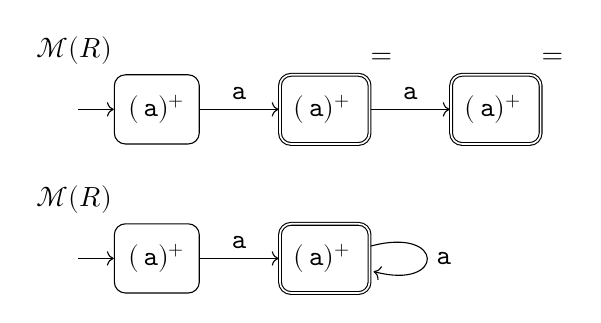
\begin{tikzpicture}
    \tikzset{
      node distance=1cm,
      every state/.style={rectangle, rounded corners, inner sep=0.5em},
      initial text=$ $,
    }
    \node[state, initial, label=above left:$\Automaton{\RE{r}}$] (u0) {$\KleenePlus{(\Pos\Char{a})}$};
    \node[state, accepting, right=of u0, label={above right:=}] (u1) {$\KleenePlus{(\Pos\Char{a})}\Pos$};
    \node[state, accepting, right=of u1, label={above right:=}] (u2) {$\KleenePlus{(\Pos\Char{a})}\Pos$};
    \draw (u0) edge[->] node[auto]{$\Char{a}$} (u1);
    \draw (u1) edge[->] node[auto]{$\Char{a}$} (u2);

    \node[state, initial, below=of u0, label=above left:$\Automaton{\RE{r}}$] (p0) {$\KleenePlus{(\Pos\Char{a})}$};
    \node[state, accepting, right=of p0] (p1) {$\KleenePlus{(\Pos\Char{a})}\Pos$};
    \draw (p0) edge[->] node[auto]{$\Char{a}$} (p1);
    \draw (p1) edge[->, loop right] node[auto]{$\Char{a}$} (p1);
  \end{tikzpicture}
\end{center}

\subsection*{Primeri}
\subsubsection{Števila}
\begin{equation*}
  \N{\RE{r}} = \KleenePlus{\{\Char{0}, \dots, \Char{9}\}}
\end{equation*}
\Next

\subsubsection{Naravna števila}
\begin{equation*}
  \Language{\N{\RE{r}}} = \{\Str{1}, \Str{2}, \dots\}
\end{equation*}
\Next

\subsubsection{Cela števila}
\begin{equation*}
  \N{\RE{r}} = (\Char{+} \Union \Char{-}) \Seq \KleenePlus{\{\Char{0}, \dots, \Char{9}\}}
\end{equation*}
\Next

\subsubsection{Heksadecimalna števila}
\begin{equation*}
  \Language{\N{\RE{r}}} = \{\Str{0x0}, \Str{0x1}, \dots, \Str{0xA}, \dots, \Str{0xFFFF}, \dots\}
\end{equation*}
\Next

\subsubsection{Barve}
\begin{equation*}
  \Language{\N{\RE{r}}} = \{\Str{\#000000}, \dots, \Str{\#FFFFFF}\}
\end{equation*}
\Next

\subsubsection{Števila s plavajočo vejico}
\begin{equation*}
  \N{\RE{r}} = (\Char{+} \Union \Char{-}) \Seq \KleenePlus{\{\Char{0}, \dots, \Char{9}\}} \Spc \Char{.} \Spc \Kleene{\{\Char{0}, \dots, \Char{9}\}}
\end{equation*}
\Next

\subsubsection{Imena spremenljivk}
\begin{equation*}
  \N{\RE{r}} = \KleenePlus{\{\Char{a}, \dots, \Char{z}\}}
\end{equation*}

\subsubsection{Ključne besede in imena spremenljivk}
\begin{align*}
  \N{\RE{r}} &= \KleenePlus{\{\Char{a}, \dots, \Char{z}\}}\\
  \N{\RE{p}} &= \Char{a} \Spc \Char{b}\\
  \N{\RE{q}} &= \Char{a} \Spc \Char{b} \Spc \Char{c}\\
  \N{\RE{t}} &= \Char{a} \Spc \Char{c} \Spc \Char{d}
\end{align*}

  \hspace*{-90px}
  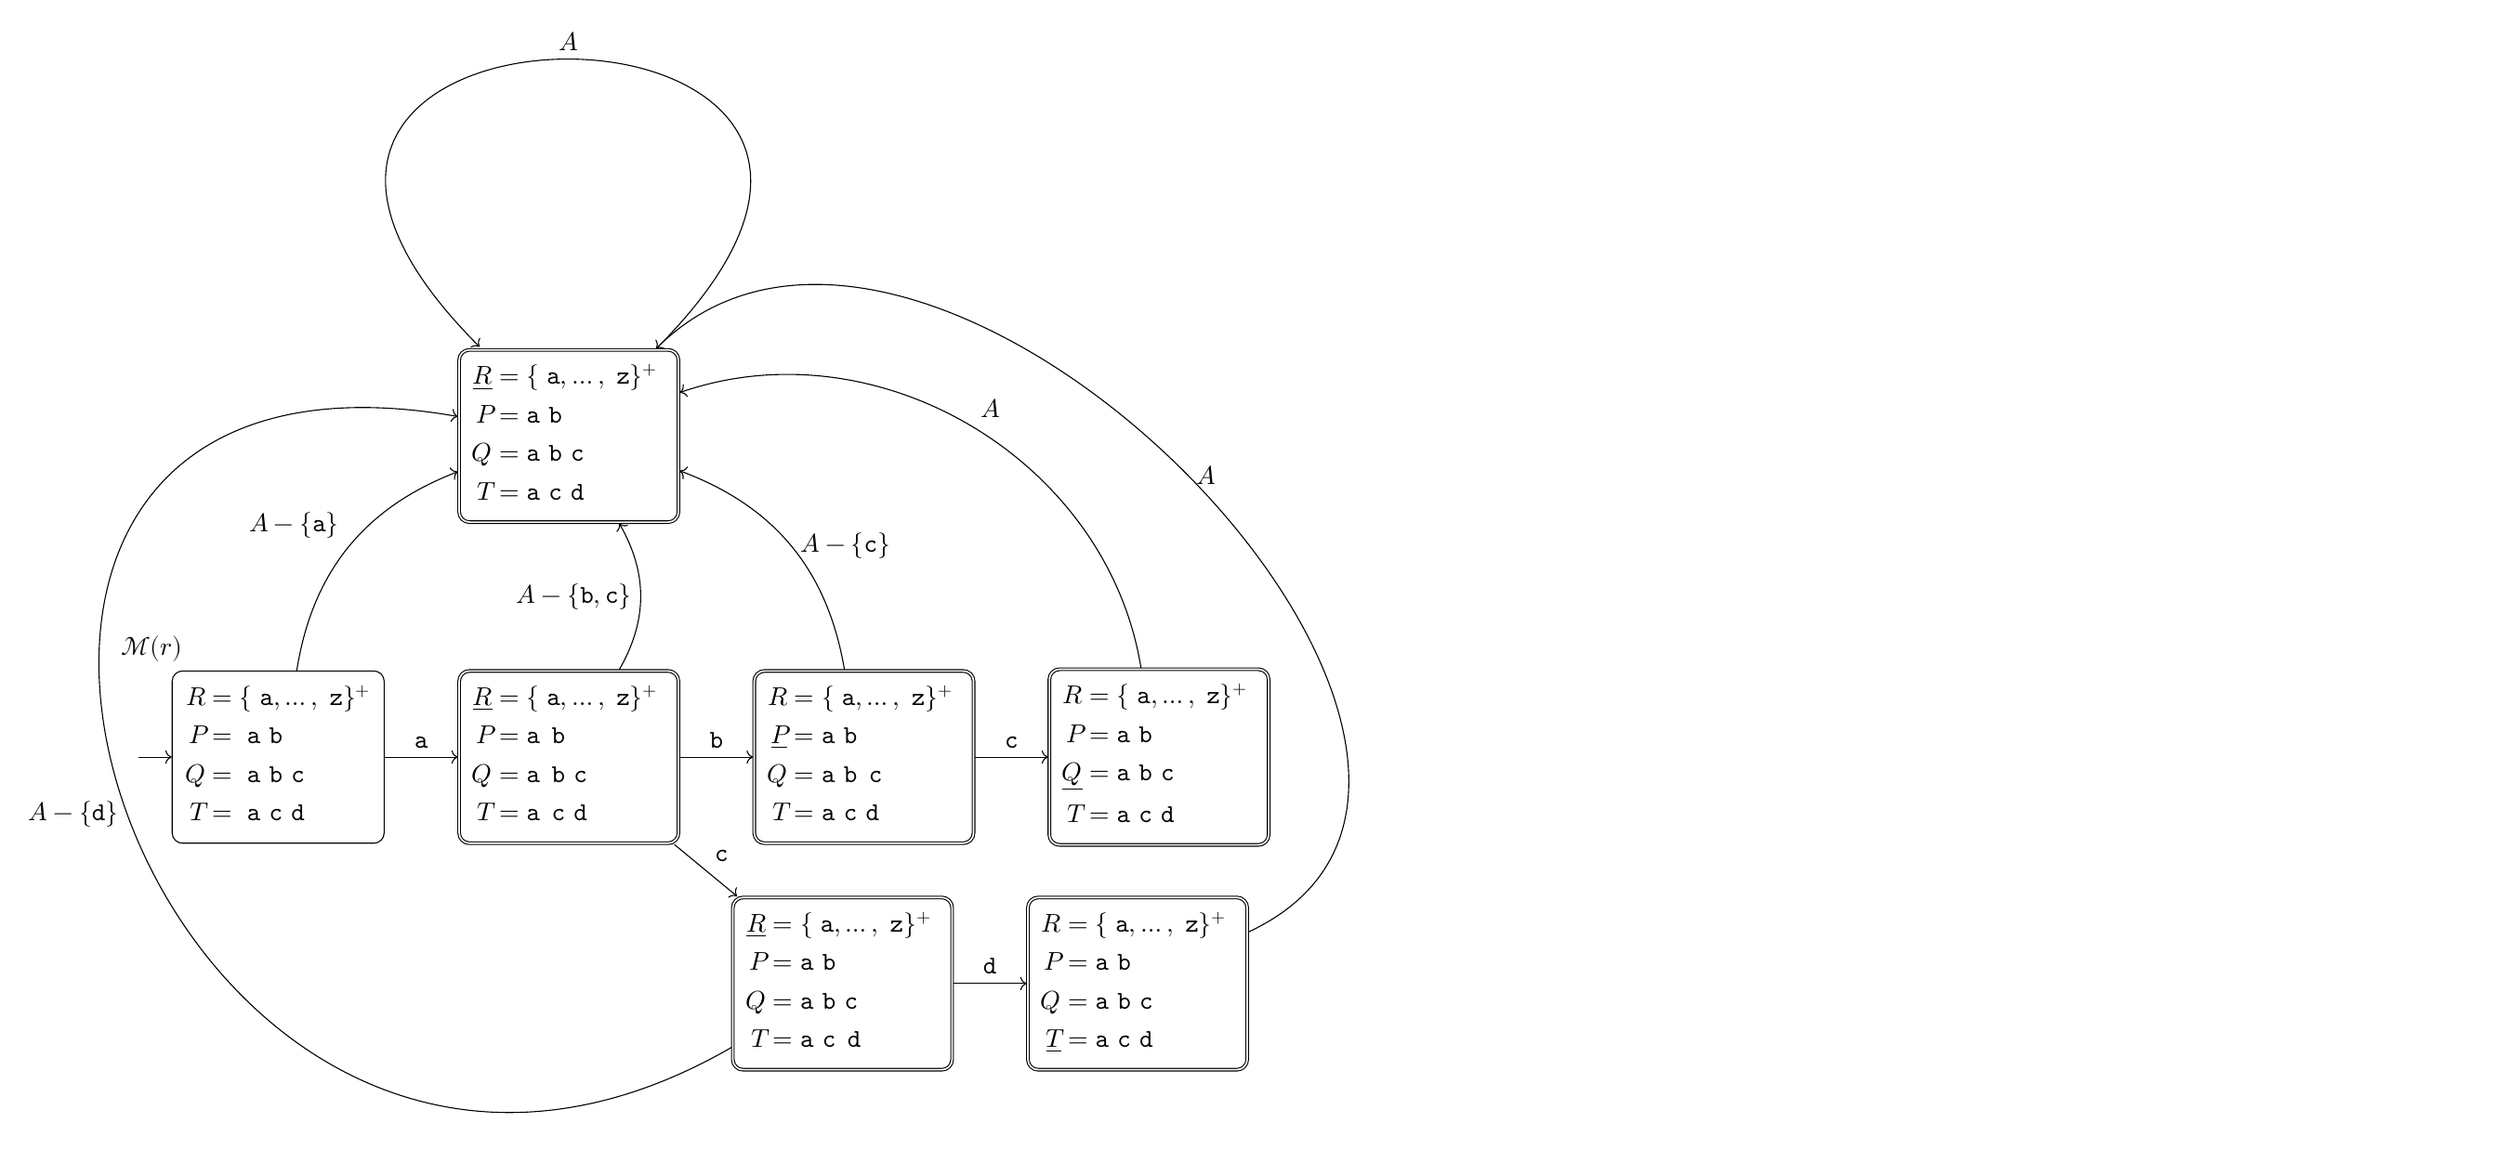
\begin{tikzpicture}
    \tikzset{
      ->,
      node distance=1cm,
      every state/.style={rectangle, rounded corners, inner sep=0.5em},
      initial text=$ $,
    }

    \clip (-3.45,-5) rectangle (30, 10);

    \node[state, initial, label=above left:$\Automaton{\N{r}}$] (v0) {$\begin{aligned}
      \N{\RE{r}} &= \KleenePlus{\{\Pos\Char{a}, \dots, \Pos\Char{z}\}}\\
      \N{\RE{p}} &= \Pos\Char{a} \Spc \Char{b}\\
      \N{\RE{q}} &= \Pos\Char{a} \Spc \Char{b} \Spc \Char{c}\\
      \N{\RE{t}} &= \Pos\Char{a} \Spc \Char{c} \Spc \Char{d}
    \end{aligned}$};

    \node[state, accepting, right=of v0] (v1) {$\begin{aligned}
      \underline{\N{\RE{r}}} &= \KleenePlus{\{\Pos\Char{a}, \dots, \Pos\Char{z}\}}\Pos\\
      \N{\RE{p}} &= \Char{a} \Pos \Char{b}\\
      \N{\RE{q}} &= \Char{a} \Pos \Char{b} \Spc \Char{c}\\
      \N{\RE{t}} &= \Char{a} \Pos \Char{c} \Spc \Char{d}
    \end{aligned}$};

    \node[state, accepting, right=of v1] (v2) {$\begin{aligned}
      \N{\RE{r}} &= \KleenePlus{\{\Pos\Char{a}, \dots, \Pos\Char{z}\}}\Pos\\
      \underline{\N{\RE{p}}} &= \Char{a} \Spc \Char{b}\Pos\\
      \N{\RE{q}} &= \Char{a} \Spc \Char{b} \Pos \Char{c}\\
      \N{\RE{t}} &= \Char{a} \Spc \Char{c} \Spc \Char{d}
    \end{aligned}$};
    \draw (v0) edge[->] node[auto]{$\Char{a}$} (v1);
    \draw (v1) edge[->] node[auto]{$\Char{b}$} (v2);

    \node[state, accepting, right=of v2] (v3) {$\begin{aligned}
      \N{\RE{r}} &= \KleenePlus{\{\Pos\Char{a}, \dots, \Pos\Char{z}\}}\Pos\\
      \N{\RE{p}} &= \Char{a} \Spc \Char{b}\\
      \underline{\N{\RE{q}}} &= \Char{a} \Spc \Char{b} \Spc \Char{c} \Pos\\
      \N{\RE{t}} &= \Char{a} \Spc \Char{c} \Spc \Char{d}
    \end{aligned}$};
    \draw (v2) edge[->] node[auto]{$\Char{c}$} (v3);

    \node[state, accepting, below right=of v1] (v4) {$\begin{aligned}
      \underline{\N{\RE{r}}} &= \KleenePlus{\{\Pos\Char{a}, \dots, \Pos\Char{z}\}}\Pos\\
      \N{\RE{p}} &= \Char{a} \Spc \Char{b}\\
      \N{\RE{q}} &= \Char{a} \Spc \Char{b} \Spc \Char{c}\\
      \N{\RE{t}} &= \Char{a} \Spc \Char{c} \Pos \Char{d}
    \end{aligned}$};

    \node[state, accepting, right=of v4] (v5) {$\begin{aligned}
      \N{\RE{r}} &= \KleenePlus{\{\Pos\Char{a}, \dots, \Pos\Char{z}\}}\Pos\\
      \N{\RE{p}} &= \Char{a} \Spc \Char{b}\\
      \N{\RE{q}} &= \Char{a} \Spc \Char{b} \Spc \Char{c}\\
      \underline{\N{\RE{t}}} &= \Char{a} \Spc \Char{c} \Spc \Char{d} \Pos
    \end{aligned}$};

    \draw (v1) edge[->] node[auto]{$\Char{c}$} (v4);
    \draw (v4) edge[->] node[auto]{$\Char{d}$} (v5);

    \node[state, accepting, above=2cm of v1] (s) {$\begin{aligned}
      \underline{\N{\RE{r}}} &= \KleenePlus{\{\Pos\Char{a}, \dots, \Pos\Char{z}\}}\Pos\\
      \N{\RE{p}} &= \Char{a} \Spc \Char{b}\\
      \N{\RE{q}} &= \Char{a} \Spc \Char{b} \Spc \Char{c}\\
      \N{\RE{t}} &= \Char{a} \Spc \Char{c} \Spc \Char{d}
    \end{aligned}$};

    \draw (v0) edge[->, bend left] node[auto]{$A - \{\Char{a}\}$} (s);
    \draw (v1) edge[->, bend right] node[auto]{$A - \{\Char{b}, \Char{c}\}$} (s);
    \draw (v2) edge[->, bend right] node[right]{$A - \{\Char{c}\}$} (s);
    \draw (v3) edge[->, bend right=50] node[above right]{$A$} (s);
    \draw (v4) edge[->, out=-150, in=170, looseness=2.5] node[left ]{$A - \{\Char{d}\}$} (s);
    \draw (v5) edge[->, out=25, in=45, looseness=1.2] node[right]{$A$} (s);
    \draw (s) edge[->, loop] node[above]{$A$} (s);
  \end{tikzpicture}

\end{document}
